\chapter{Test on simulated Data}
	
	\section{Fixed Community representation}
	
	We draw a simulation of a network with $n = 25$, $ p = 3$, $k = 4$, $a = 2$, $b = 2$, optimized it. We obtain the graph with ranking gap of 5.83 for a mean of 8.32 and AE of 0.013
	\begin{figure}[H]
		\centering
		%		\textbf{Your title}\par\medskip
		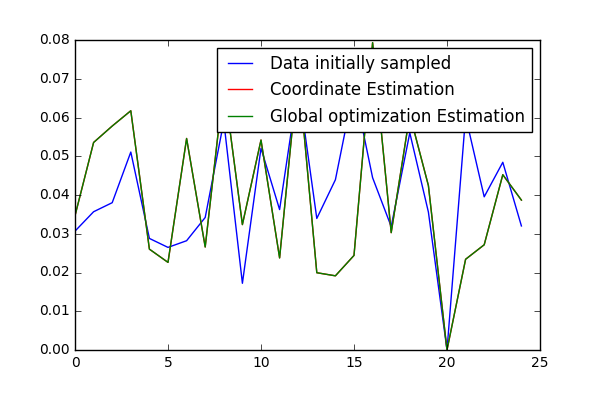
\includegraphics[width=\textwidth,height=\textheight,keepaspectratio]{LambdaEstimationFixedPrior}
		\caption{Lambda Estimation Fixed Prior}
		\label{label-image9}
	\end{figure}
	\begin{figure}[H]
		\centering
		\begin{subfigure}[b]{0.55\textwidth}
			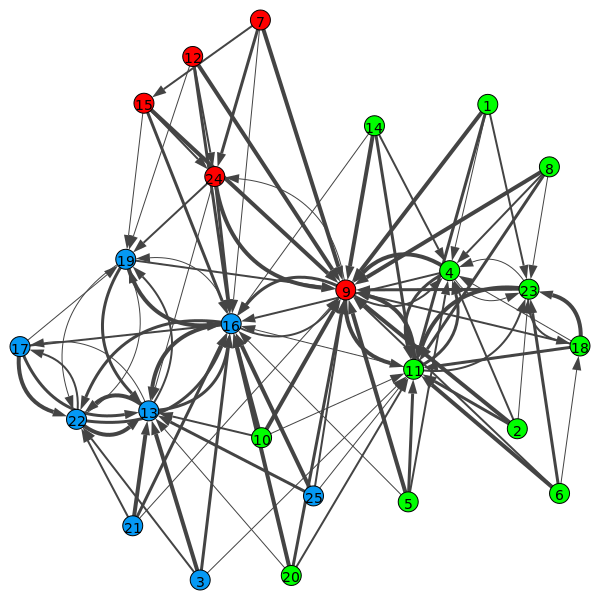
\includegraphics[width=1\linewidth]{OriginalPlotFixedPrior}
			\caption{}
			\label{fig:Ng1} 
		\end{subfigure}
		
		\begin{subfigure}[b]{0.55\textwidth}
			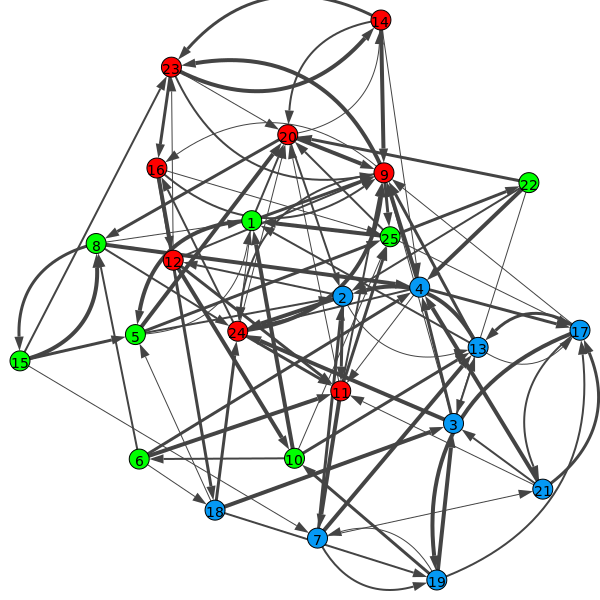
\includegraphics[width=1\linewidth]{OptimizationPlotFixedPrior}
			\caption{}
			\label{fig:Ng2}
		\end{subfigure}
		
		\caption[Two graphs]{(a) Original Graph. (b) Inferred Graph}
	\end{figure}
	Now we made a simulation of 10 networks and measured the mean Absolute Error and Ranking Gap.
	We have a mean ranking gap of $2.8871111111111114$ compared to a mean of 5. A a mean AE of $0.022484955968703896$
	
	We run for 100 networks with the same parameters.
	We have mean ranking gap of 2.9304888888888896 and mean AE of 0.02122157183931606
	\begin{figure}[H]
		\centering
		\begin{minipage}{0.45\textwidth}
			\centering
			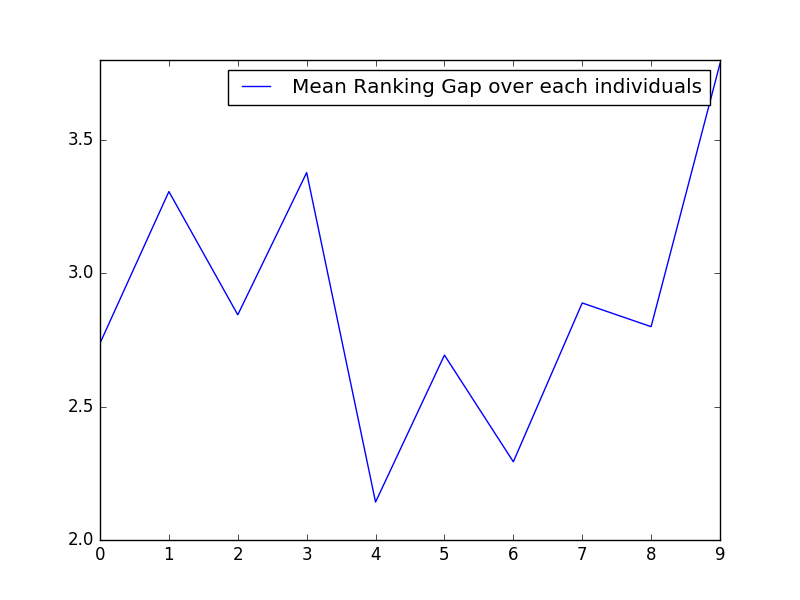
\includegraphics[width=0.9\textwidth]{SimulationGap} % first figure itself
			\caption{Ranking Gap Community Representation for $10$ networks}
			\label{label-image12}
		\end{minipage}\hfill
		\begin{minipage}{0.45\textwidth}
			\centering
			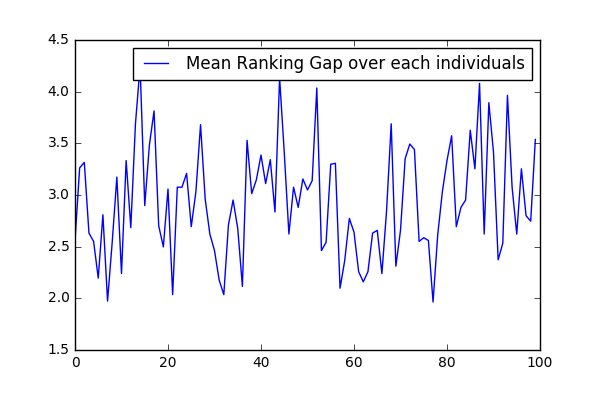
\includegraphics[width=0.9\textwidth]{SimulationGap100} % second figure itself
			\caption{Ranking Gap Community Representation for $100$ networks}
			\label{label-image13}
		\end{minipage}
	\end{figure}
	
	\section{Model With Degree Correction}
	
	We draw a simulation of 100 networks with $n = 100$, $ p = 3$, $k = 4$, $a = 2$, $b = 2$, optimized it. We obtain the graph with ranking gap of 2.942666666666666 for a mean of 5 and AE of 0.03798207013695899
	
	\begin{figure}[H]
		\centering
		%		\textbf{Your title}\par\medskip
		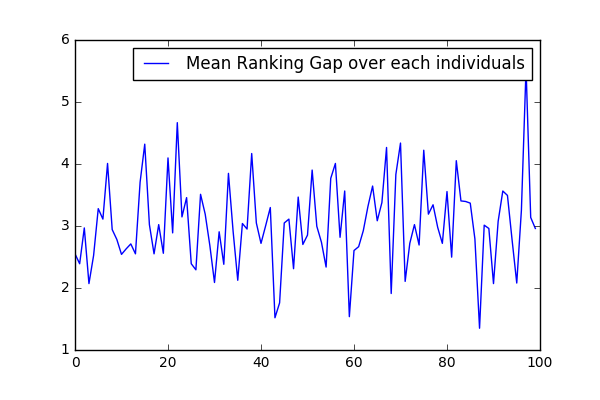
\includegraphics[width=\textwidth,height=\textheight,keepaspectratio]{SimulationGapDegreeCorr}
		\caption{Ranking Gap Degree Correction}
		\label{label-image14}
	\end{figure}
	
	
	\section{Model With Covariates}
	
	We simulated 100 networks of 100 individuals with the rank model:
	
	$y_{i,j} = \beta_{0} + a_{i} + b_{j} + \epsilon_{i,j}$
	
	
	\(
	\begin{pmatrix}
	a_{i} \\
	b_{i}
	\end{pmatrix}
	\), i = 1,...,n $\sim $ i.i.d normal(0,$\Sigma_{ab}$)
	
	\(
	\begin{pmatrix}
	\epsilon_{i,j} \\
	\epsilon_{j,i}
	\end{pmatrix}
	\), i = 1,...,n $\sim $ i.i.d normal(0,$\sigma^{2}$ $\begin{pmatrix} 1 & \rho \\ \rho & 1 \end{pmatrix}$)
	
	
	
	
	\chapter{Simulations on the Sampson’s monk dataset}
	In this part we use the The data set collected by Sampson (1968) this is a classic data set in social network analysis. The data set summarizes relationships, observed at three distinct time points, among 18 monks who were about to enter a monastery when a conflict erupted. We use here the directed network where $y_{i,j} = 1$ denotes that monk $i$ ranked monk $j$ among his top three preferred individuals and $y_{i,j} = 0$ otherwise. The directed network is shown in Figure \ref{label-image4} , where circles represent monks and directed edges are oriented from $i$ to $j$ whenever $y_{i,j} = 1$. The monks are divided by Sampson into three groups: Loyal Opposition, Turks, and Outcasts.
	
	We applied the same method as for the simulated data and obtained the following community. We can observe that our model identifies exactly the same clustering of communities as the ones observed by Sampson. Namely the Loyal Opposition (Red community), Turks (Green Community), and Outcasts (Blue Community). In this graph the individuals are labeled according to their number provided with their names in the data set package and not according to their rank in the data-frame.
	
	
	\begin{figure}
		\centering
		%		\textbf{Your title}\par\medskip
		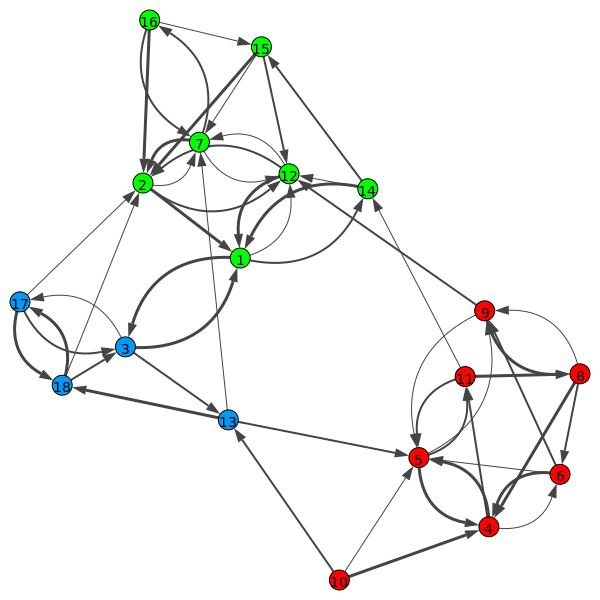
\includegraphics[width=\textwidth,height=\textheight,keepaspectratio]{OptimizationPlotSam}
		\caption{Inferred community for the Sampson DataSet}
		\label{label-image4}
	\end{figure}